\documentclass[11pt]{extarticle}
\usepackage[margin=2.5cm]{geometry}
\usepackage[T1]{fontenc} 
\usepackage[french]{babel}
\usepackage{mathptmx} % Times New Roman
\usepackage{amsthm}
\usepackage{graphicx}
\usepackage{booktabs}  % Pour de meilleurs tableaux
\usepackage{microtype} % Pour une meilleure typographie
\usepackage{xcolor}    % Pour la couleur
\usepackage{hyperref}  % Pour les liens cliquables
\usepackage{fancyhdr} % Pour personnaliser les en-têtes
\usepackage{enumitem} % Pour personnaliser les listes
\usepackage{caption}  % Pour personnaliser les légendes
\usepackage{float}    % Pour un meilleur contrôle du placement des figures
\usepackage{xcolor,colortbl}
\usepackage{eso-pic}


% Configuration des couleurs et des liens
\hypersetup{
    colorlinks=true,
    linkcolor=blue,
    filecolor=magenta,
    urlcolor=cyan,
}

\newcommand{\HRule}{\rule{\linewidth}{0.5mm}}
\newcommand{\blap}[1]{\vbox to 0pt{#1\vss}}
\newcommand\AtUpperLeftCorner[3]{%
  \put(\LenToUnit{#1},\LenToUnit{\dimexpr\paperheight-#2}){\blap{#3}}%
}
\newcommand\AtUpperRightCorner[3]{%
  \put(\LenToUnit{\dimexpr\paperwidth-#1},\LenToUnit{\dimexpr\paperheight-#2}){\blap{\llap{#3}}}%
}

% Configuration des en-têtes
\pagestyle{fancy}
\fancyhf{}
\fancyhead[L]{\leftmark}
\fancyhead[R]{\thepage}
\renewcommand{\headrulewidth}{0.4pt}

% Titre personnalisé
\title{Étude Comparative des Moteurs de Stockage}
\date{Octobre 2024}
\author{Bernard-Bodier Léo | Bodin Grégoire}

\makeatletter


\begin{document}

\enlargethispage{2cm}

\AddToShipoutPicture{
        \AtUpperLeftCorner{1.5cm}{1.8cm}{
\includegraphics[width=6cm]{images/logoistic.png}}
        \AtUpperRightCorner{1.5cm}{1cm}{
\includegraphics[width=6cm]{images/LogoRennes1.png}
    }
}
\begin{center}
    \vspace*{7cm}
    \HRule\\
    \vspace{0.5cm}
    \huge
    \textbf{{\@title}}
    \HRule
    \vspace*{0.5cm}
    \Large{\@date}
    \\
    \Large{\@author} 
\end{center}
\vspace{12cm}
leo.bernard--bodier@etudiant.univ-rennes.fr
\hfill
gregoire.bodin@etudiant.univ-rennes.fr

\thispagestyle{empty}
\newpage
\ClearShipoutPicture

\tableofcontents
\thispagestyle{empty}
\newpage

\section{Introduction}

\subsection{Contexte et Définitions}
\paragraph{}
Une \textbf{base de données} est un ensemble structuré d'informations organisées de manière à être facilement accessibles, gérées et mises à jour. Elle constitue le fondement de nombreux systèmes d'information modernes, permettant aux organisations de stocker, gérer et assurer la cohérence d'un grand volume de données.

\subsection{Lien vers le dépôt GitHub}
\paragraph{}
Vous pouvez accéder au code source complet de ce projet sur GitHub en suivant ce lien : \href{https://github.com/GregoireBDN/Database-Analyzer}{GitHub - Database Analyzer}.

\subsection{Choix du Sujet}

\begin{figure}[H]
    \centering
    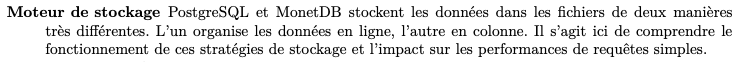
\includegraphics[width=1\textwidth]{images/Sujet.png}
    \label{fig:sujet}
\end{figure}

\subsection{Présentation des SGBD}

\paragraph{} 
MonetDB et PostgreSQL sont deux systèmes de gestion de base de données (SGBD). Ils sont tous deux relationnels, c'est-à-dire que les données sont stockées dans des tables, qui sont reliées les unes aux autres.

\paragraph{} 
\textbf{MonetDB} : Développé dans les années 1990 par un institut de recherche des Pays-Bas, l'objectif de ce système de gestion est de répondre aux besoin d'analyses croissantes des entreprises en créant une application performante et novatrice.

\paragraph{} 
\textbf{PostgreSQL} : Développé en 1986 en Californie par un professeur de l'université et son équipe, c'est un projet open source, maintenu à jour par une vaste communauté de développeurs à travers le monde. Sa fiabilité à gérer des base de données complexes et sa flexibilité ont fait de PostgreSQL l'un des SGDB les plus utilisés dans le monde.

\subsection{Problématique}
\paragraph{}
L'évolution des bases de données reflète les défis changeants du stockage et de l'analyse des données :

\subsubsection{Évolution Historique}

Dans les années 1950-1960, les premiers systèmes de stockage hiérarchiques émergent, avec l'introduction du terme "Data Base" en 1964, marquant un tournant dans la gestion des données. 
\paragraph{} Dans les années 1970-1980, les bases de données relationnelles deviennent prédominantes, favorisant le modèle orienté lignes qui structure l’information de manière efficace pour les transactions. 
\paragraph{} Les années 1990-2000 sont marquées par une croissance exponentielle des volumes de données, augmentant la demande pour des analyses complexes, tout en révélant les limites du modèle orienté lignes pour les besoins analytiques. 
\paragraph{} Enfin, entre 2000 et 2020, les bases orientées colonnes émergent pour répondre à ces défis, entraînant une coexistence entre les modèles orientés lignes et colonnes, chacun ayant ses propres avantages selon les cas d'utilisation.


\subsubsection{Enjeux Actuels}
\paragraph{}
La coexistence de ces deux approches soulève plusieurs questions essentielles. D'abord, il est crucial d'examiner les \textbf{performances} relatives selon le type de requête, car chaque méthode peut offrir des avantages distincts selon le contexte. Ensuite, la \textbf{volumétrie} des données joue un rôle déterminant : comment le volume influence-t-il les performances et la réactivité du système ?  Par ailleurs, le choix du modèle à privilégier doit être basé sur le \textbf{cas d'utilisation spécifique}, afin d'optimiser l'efficacité. Enfin, \textbf{l'hybridation} des deux approches mérite d'être considérée : est-il pertinent de les combiner pour tirer parti des forces de chacune et répondre ainsi aux besoins variés des utilisateurs ?

\section{Architectures de Stockage}

\subsection{Bases de Données Orientées Lignes}
\paragraph{}
Le modèle orienté lignes s’est rapidement imposé dans les premiers systèmes de gestion de bases de données en raison de plusieurs avantages clés. Tout d’abord, il s’adapte parfaitement aux opérations CRUD (Create, Read, Update, Delete), ce qui en fait un choix évident pour la gestion des données. De plus, ce modèle s'avère particulièrement efficace pour les transactions qui impliquent des enregistrements complets, garantissant une manipulation rapide et fluide des données. Sa facilité d’implémentation et de compréhension contribue également à sa popularité, permettant aux développeurs de l’adopter sans difficulté. Enfin, il offre une performance optimale pour les applications transactionnelles, où la rapidité et la fiabilité sont essentielles.

\subsubsection{Exemple de Structure}
\begin{table}[H]
    \centering
    \begin{tabular}{|c|c|c|c|}
    \hline
    \textbf{ID} & \textbf{Prénom} & \textbf{Nom} & \textbf{Âge} \\
    \hline
    1 & Léo & Bernard-Bodier & 22 \\
    2 & Grégoire & Bodin & 21 \\
    3 & Macéo & Dapsance & 22 \\
    \hline
    \end{tabular}
    \caption{Structure d'une base de données orientée lignes}
    \label{tab:row_oriented}
\end{table}


\subsubsection{Stockage Physique}
\noindent\textbf{Format de stockage sur le disque :}\\
\texttt{(1,Léo,Bernard-Bodier,22)(2,Grégoire,Bodin,21)(3,Macéo,Dapsance,22)}

\subsection{Bases de Données Orientées Colonnes}

\paragraph{}    L’émergence des bases orientées colonnes répond à des besoins croissants liés à l’analyse de grands volumes de données. Ce modèle est particulièrement adapté aux requêtes ciblant des attributs spécifiques, permettant des accès plus rapides et plus efficaces. De plus, il optimise l’espace de stockage grâce à des techniques de compression, réduisant ainsi l’empreinte mémoire. Enfin, les bases orientées colonnes offrent une amélioration significative des performances pour les requêtes analytiques, ce qui en fait un choix privilégié pour les applications nécessitant des analyses complexes et des traitements de données à grande échelle.

\subsubsection{Exemple de Structure}
\begin{table}[H]
    \centering
    \begin{tabular}{|c|c|c|c|}
    \hline
    \textbf{ID} & 1 & 2 & 3 \\
    \hline
    \textbf{Prénom} & Léo & Grégoire & Macéo \\
    \hline
    \textbf{Nom} & Bernard-Bodier & Bodin & Dapsance \\
    \hline
    \textbf{Âge} & 22 & 21 & 22 \\
    \hline
    \end{tabular}
    \caption{Structure d'une base de données orientée colonnes}
    \label{tab:column_oriented}
\end{table}

\subsubsection{Stockage Physique}
\noindent\textbf{Format de stockage sur le disque :}\\
\texttt{(1,2,3)(Léo,Grégoire,Macéo)(Bernard-Bodier,Bodin,Dapsance)(22,21,22)}

\subsection{Vue d'ensemble des Approches}

\begin{figure}[H]
    \centering
    \begin{tabular}{|p{0.45\textwidth}|p{0.45\textwidth}|}
    \hline
    \textbf{Orienté Lignes} & \textbf{Orienté Colonnes} \\
    \hline
    Optimal pour transactions & Optimal pour analyses \\
    Accès rapide aux enregistrements complets & Accès rapide aux attributs spécifiques \\
    Insertion/mise à jour efficaces & Agrégations performantes \\
    Stockage séquentiel des données & Compression efficace des données \\
    \hline
    \end{tabular}
    \caption{Comparaison des caractéristiques principales des deux approches}
    \label{tab:comparison}
\end{figure}

\section{Analyse théorique des requêtes}
\paragraph{}
Peu importe si vous utilisez PostgreSQL ou bien MonetDB, vous serez en mesure de réaliser les requêtes que vous souhaitez. Cependant, ces systèmes permettent d'être plus ou moins performant selon certains critères comme le type de requête mais aussi la taille du jeu de donnée.

\subsection{Petits jeux de données}
\paragraph{}
 Lorsqu'on manipule des jeux de données relativement petits, \textbf{PostgreSQL} offrira des meilleurs performances dans tous les types de requêtes. En effet grâce à son architecture de stockage en lignes, il permet un accès facile et rapide aux informations complètes d'une entrée. Les caches sont optimisés de sorte à ce que le plus de données possible soient stockées sur la RAM plutôt que sur le disque, ce qui réduit encore considérablement la latence des requêtes.

\subsection{Grands jeux de données}
\paragraph{}
En ce qui concerne les très grands ensembles de données, on va s'intéresser à chaque type de requête plus en profondeur car c'est dans ces conditions que des différences vont être observables entre les 2 SGDB.

\subsubsection{Sélections}
\paragraph{}
\textbf{MonetDB} sera le plus performant des deux sur les sélections simples. Son stockage en colonnes réduit le nombre de données à scanner pour chaque colonne présente dans la requête.

\subsubsection{Agrégation (SUM, AVG, COUNT)}
\paragraph{}
Ici aussi, \textbf{MonetDB} est plus efficace car son moteur permet de traiter des colonnes entières en parallèles. Il est ainsi beaucoup plus performant que son concurrent dans ce type scénarios.

\subsubsection{Jointures}
\paragraph{}
Une fois de plus, c'est \textbf{MonetDB} qui est susceptible d'être le plus rapide. Il permet des jointures complexes sans pour autant avoir à traiter chaque ligne complète.

\subsubsection{Mise à Jour (UPDATE)}
\paragraph{}
\textbf{PostgreSQL} reste plus performant ici car il n'a pas besoin de changer la colonne entière avec son stockage en lignes. Contrairement à MonetDB qui, à chaque update doit reconstruire toutes les colonnes impliquées.

\subsubsection{Insertions}
\paragraph{}
Une nouvelle fois \textbf{PostgreSQL} est plus rapide. En effet, il optimise les transactions pour une gestion efficace des nouvelles entrées.


\subsubsection{Analyse de Données}
\paragraph{}
\textbf{MonetDB} se distingue grâce a son stockage en colonne ainsi qu'à son moteur de requêtes optimisé pour offrir une capacité d'analyse performante, même pour des millions d'entrées.

\subsubsection{Indexation}
\paragraph{}
Enfin, \textbf{PostgreSQL} est le meilleur choix car ses options d'indexations sont plus rapides, et il supporte plus de possibilités.

\subsection{Récapitulatif}

\begin{table}[ht]
    \centering
    \setlength\arrayrulewidth{1pt}
    \def\arraystretch{0.82}
    \begin{tabular}{|l|c|c|}
    \hline
         \textbf{Requêtes} &  \textbf{PostgreSQL}
         & \textbf{MonetDB} \\ \hline
         \rowcolor[HTML]{343434} 
                    {\color[HTML]{FFFFFF} \textbf{Petit jeu de données}} &  & \\ \hline
                    Sélections & \cellcolor[HTML]{FCBF01}X &  \\ \hline
                    Agrégations & \cellcolor[HTML]{FCBF01}X &  \\ \hline
                    Jointures & \cellcolor[HTML]{FCBF01}X &  \\ \hline
                    Mises à jour & \cellcolor[HTML]{FCBF01}X &  \\ \hline
                    Insertions & \cellcolor[HTML]{FCBF01}X &  \\ \hline
                    Analyses & \cellcolor[HTML]{FCBF01}X &  \\ \hline
                    Indexation & \cellcolor[HTML]{FCBF01}X &  \\ \hline
                    \rowcolor[HTML]{343434} 
                    {\color[HTML]{FFFFFF} \textbf{Grand jeu de données}} &  & \\ \hline
                    Sélections &  & \cellcolor[HTML]{32C423}X  \\ \hline
                    Agrégations &  & \cellcolor[HTML]{32C423}X \\ \hline
                    Jointures &  & \cellcolor[HTML]{32C423}X \\ \hline
                    Mises à jour & \cellcolor[HTML]{FCBF01}X &  \\ \hline
                    Insertions & \cellcolor[HTML]{FCBF01}X &  \\ \hline
                    Analyses &  & \cellcolor[HTML]{32C423}X \\ \hline
                    Indexation & \cellcolor[HTML]{FCBF01}X &  \\ \hline
                    
                    
    \end{tabular}
    \caption{Comparatif des performances en fonction des requêtes entre PostgreSQL et MonetDB}
    \label{tab:my_label}
\end{table}



\subsection{Conclusion}
\paragraph{}
Pour résumer, PostgreSQL sera plus performant pour les petits jeux de données grâce à son architecture orientée lignes et ses optimisations pour les requêtes rapides. En revanche, pour les bases de données volumineuses, le choix dépend du type de requête. En effet MonetDB excelle dans les requêtes analytiques et les agrégations, tandis que PostgreSQL reste plus efficace pour les opérations transactionnelles comme les mises à jour et les insertions.

\section{Démarches à venir}
\paragraph{}
Lors de la phase expérimentale, nous allons nous concentrer sur les sélections et les agrégations.

\subsection{Jeu de données}
\paragraph{}
Nous allons commencer par remplir deux jeux de données : le premier avec quelques milliers d'entrées. un jeu avec quelques centaines de données serait trop petit et ne serait pas forcément représentatif d'une base de donnée qui pourrait exister dans une entreprise avec un petit projet. De plus nous serions limités pour certains tests. Le second jeu de données contiendra quelques millions d'entrées. Ainsi nous aurons une belle différence entre le nombre d'entrées du premier jeu et celui du second jeu de données. Nous pourrons donc être sûrs que la taille des entrées est bien LE paramètre qui fera varier les résultats.

\subsection{Types de mesures}
\paragraph{}
Lors de nos tests, nous allons comparer différentes mesures pour déterminer quel SGBD est le plus optimal pour notre requête.

\subsubsection{Temps d'exécution}
\paragraph{}
Le premier critère et le plus évident est le temps d'exécution. Plus la requête met du temps à aboutir, moins le SGBD est performant pour ce type de requête.

\paragraph{}
Pour l'analyser avec PostgreSQL nous pourront utiliser "EXPLAIN ANALYZE" devant notre requête, qui nous permettra de récupérer en sortie, pour chaque étape de la requête, le coût, le nombre de lignes traitées, et le temps mis par le système.

\paragraph{}
Avec MonetDB, nous pourrons utiliser "timer start" juste avant puis "timer stop" à la fin de la requête. Ainsi nous aurons le temps total écoulé. En revanche nous n'aurons pas plus d'informations concernant les étapes de la requête.

\subsubsection{Utilisation de la RAM}
\paragraph{}
L'utilisation de la mémoire du pc peut être un bon indicateur de performances. Sur linux, on peut par exemple utiliser la commande "top" dans le terminal pour avoir accès à ces informations.

\subsubsection{Temps d'accès au cache}
\paragraph{}
Lors de l'exécution d'une requête pour la première fois, nous vérifierons bien le temps mis par celle-ci. Lors de la ré-exécution de cette même requête, nous pourrons ainsi voir si les SGBD qu'on utilise optimisent l'accès au cache ou non.

\subsubsection{Utilisation du CPU}
\paragraph{}
Enfin, on peut mesurer la charge CPU pour voir si l'un des SGBD utilise plus de ressources qu'un autre. Encore une fois, l'utilisation de la commande "top" dans le cmd pourra sûrement se montrer utile.

\subsection{Méthodologie}
\paragraph{}
Après avoir créé notre jeu de données, nous procéderons à l'exécution d'une requête une centaine de fois sur chaque modèle de base de données, afin d'éviter d'éventuelles mesures extrêmes qui pourraient fausser nos conclusions. À chaque exécution, nous allons collecter des données détaillées sur le plan d'exécution et le temps d'exécution de la requête. Toutes ces informations seront ensuite stockées dans un fichier, ce qui facilitera l'analyse des résultats. 
\paragraph{}
Ce processus nous permettra de comparer les deux systèmes de gestion de bases de données selon différentes métriques. Ainsi, nous pourrons obtenir une vision claire et précise des performances de chaque modèle dans des conditions réelles d'utilisation. Cette méthodologie pourra être répétée avec les différentes requêtes (cf. partie 3).
\paragraph{}
Pour s'assurer de la cohérence de nos mesures, nous pourrons faire l'expérimentation sur plusieurs machines avec différentes configurations et différents systèmes d'exploitation afin de s'assurer que les mesures restent identiques.

\vspace{1cm} % Espace vertical avant la ligne

% Ligne avec titre au milieu
\noindent
\makebox[\linewidth]{\rule{0.4\linewidth}{0.4pt} \hspace{1em} \textbf{PARTIE EXPERIMENTALE} \hspace{1em} \rule{0.4\linewidth}{0.4pt}}

\vspace{1cm} % Espace vertical après la ligne

\addcontentsline{toc}{section}{Partie expérimentale}
\section{Choix partie expérimentale}

\subsection{Base de données}
\paragraph{}
Nous avons sélectionné deux ensembles de données provenant de sources fiables pour nos expérimentations. Ces ensembles de données ont été choisis pour leur pertinence et leur taille, permettant une analyse comparative efficace entre PostgreSQL et MonetDB.

\subsubsection{Petite base de données}
\paragraph{}
Pour la petite base de données, nous avons choisi les données de qualité de l'air de New York, disponibles sur \href{https://catalog.data.gov/dataset/air-quality}{NYC Open Data - Air Quality}. Ce jeu de données contient environ 18 000 entrées et présente les anomalies dans l'air de la ville de New York depuis le début du 21ème siècle.

\subsubsection{Grande base de données}
\paragraph{}
Pour la grande base de données, nous avons opté pour les données de criminalité de Los Angeles, disponibles sur \href{https://catalog.data.gov/dataset/crime-data-from-2020-to-present}{LA City - Crime Data 2020 to Present}. Ce jeu de données recense tous les crimes d'un département de police de Los Angeles depuis 2020 et contient près d'un million d'entrées.


\subsection{Python et Docker}
\paragraph{}
Pour automatiser l'initialisation des bases de données, nous utilisons des scripts Python. Python est choisi pour sa flexibilité et ses bibliothèques robustes pour la gestion des bases de données. De plus, Docker est utilisé pour créer des environnements isolés, bien que des problèmes initiaux aient été rencontrés avec MonetDB sur macOS. Finalement, Docker a été intégré pour sa capacité à simplifier le déploiement et la configuration des services.

\subsection{Résultats expérimentaux}
\paragraph{}
Durant la partie théorique, nous pensions que MonetDB serait plus performant seulement dans le grand jeu de données ET pour les requêtes d'analyses, type sélections, agrégations et jointures.

\section{Petit jeu de données}
\subsection{Analyse}
\paragraph{}
Pour le petit jeu de données, nous avons utilisé les données de qualité de l'air de New York. L'analyse a montré que PostgreSQL est plus efficace pour le chargement initial des données, avec un temps de chargement de 0.03 ms par ligne, comparé à 0.22 ms par ligne pour MonetDB. Les performances des requêtes de sélection et d'agrégation étaient similaires entre les deux SGBD, mais MonetDB a montré des performances inférieures sur les jointures complexes, avec un temps d'exécution environ 7 fois plus élevé que PostgreSQL.

\subsection{Chiffres}
\paragraph{}
Voici un résumé des ordres de grandeurs (en ms/ligne pour le chargement de données et en ms pour la requête pour les 3 autres) des performances pour le petit jeu de données :


\begin{table}[ht]
    \centering
    \setlength\arrayrulewidth{1pt}
    \def\arraystretch{0.82}
    \begin{tabular}{|l|c|c|}
    \hline
         \textbf{Requêtes} &  \textbf{PostgreSQL}
         & \textbf{MonetDB} \\ \hline
         \rowcolor[HTML]{343434} 
                    {\color[HTML]{FFFFFF} \textbf{Air quality}} &  & \\ \hline
                    Chargement des données & \cellcolor[HTML]{FCBF01}0.03 &0.22  \\ \hline
                    Sélections (Q1) &1.00 &1.00 \\ \hline
                    Agrégations (Q2) &1.00 &1.00 \\ \hline
                    Jointures complexes (Q3) & \cellcolor[HTML]{FCBF01}11.00 & 72.00 \\ \hline
                    
                    
    \end{tabular}
    \caption{Comparatif des performances en fonction des requêtes entre PostgreSQL et MonetDB}
    \label{tab:my_label2}
\end{table}

\subsection{Graphes}
\paragraph{}
Les graphiques générés montrent que PostgreSQL est plus performant pour les opérations de chargement et les jointures complexes dans le petit jeu de données. En ce qui concerne les sélections et agrégations, la différence est négligeable, on peut donc considérer que les deux SGBD sont sensiblement équivalentes.

  \begin{figure}[H]
      \centering
      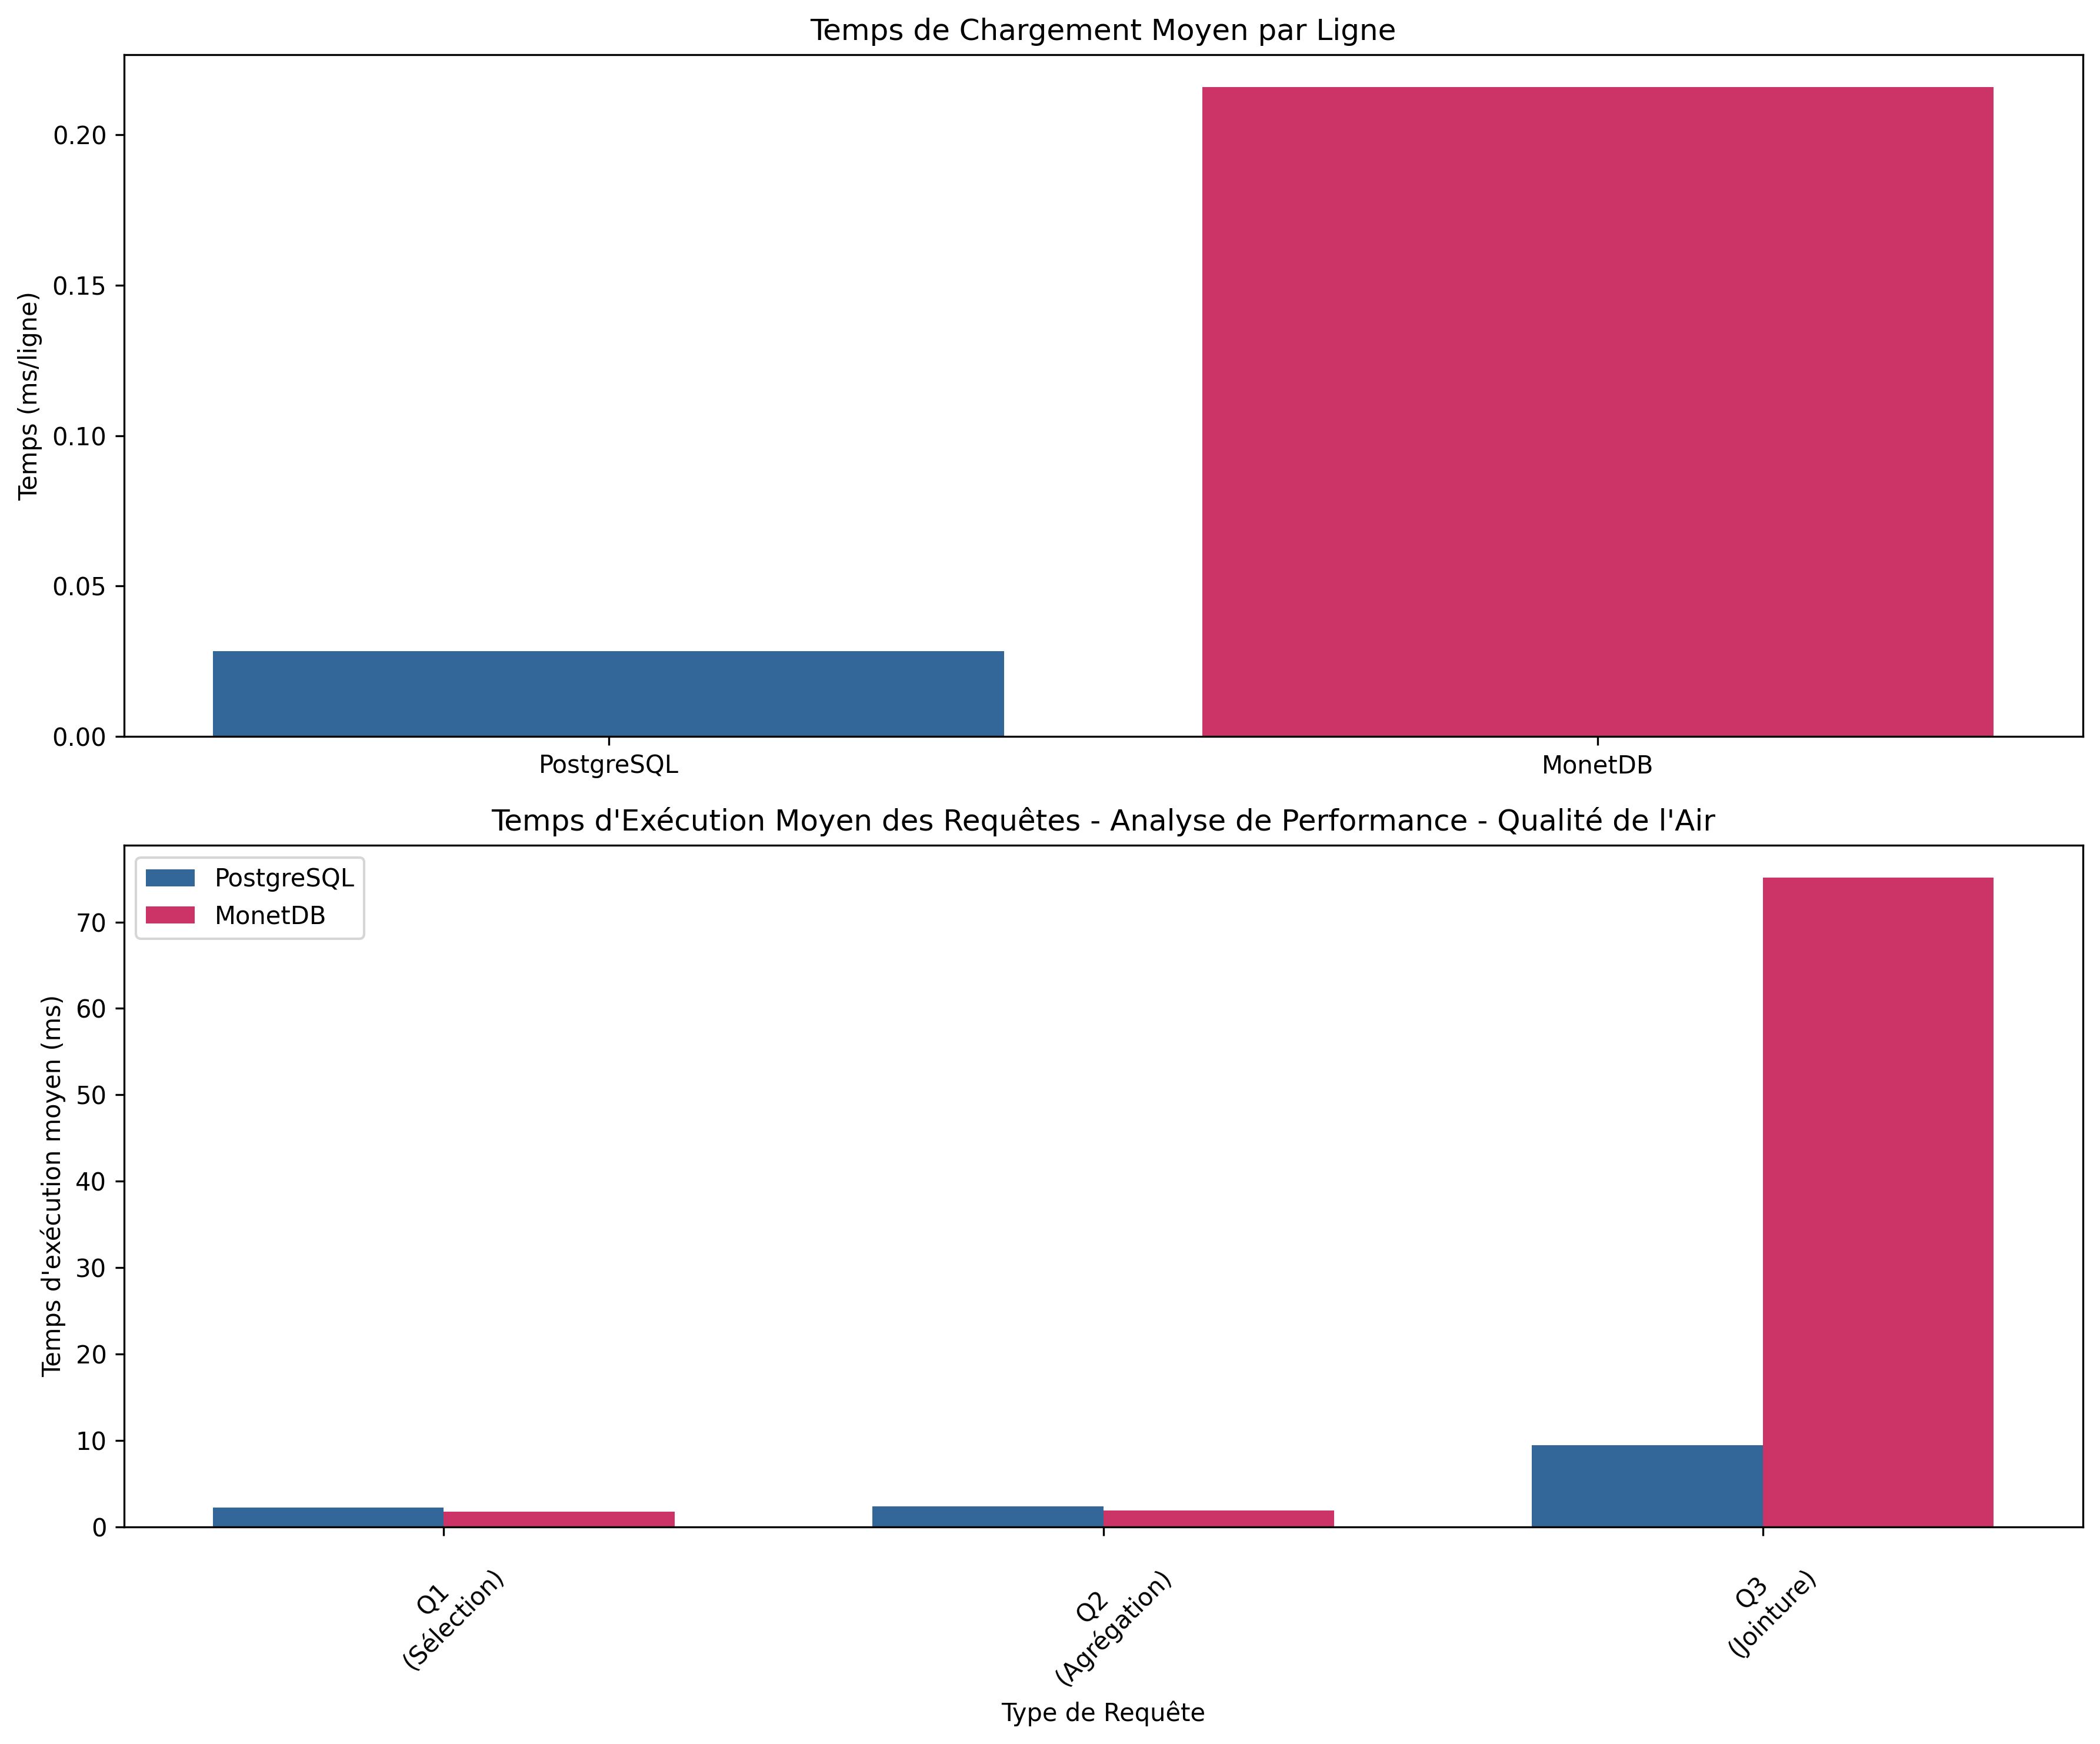
\includegraphics[width=0.8\textwidth]{images/air_quality_performance.png}
      \caption{Analyse de Performance - Qualité de l'Air}
      \label{fig:performance_air_quality}
  \end{figure}

\section{Grand jeu de données}
\subsection{Analyse}
\paragraph{}
Pour le grand jeu de données, nous avons utilisé les données de criminalité de Los Angeles. MonetDB a montré un temps de chargement plus élevé, à 0.37 ms par ligne, comparé à 0.05 ms par ligne pour PostgreSQL. Cependant, MonetDB a surpassé PostgreSQL dans les requêtes de sélection, d'agrégation et de jointure, avec des temps d'exécution significativement plus bas.

\subsection{Chiffres}
\paragraph{}
Voici un résumé des ordres de grandeurs (en ms/ligne pour le chargement de données et en ms pour la requête pour les 3 autres) des performances pour le grand jeu de données :

\begin{table}[ht]
    \centering
    \setlength\arrayrulewidth{1pt}
    \def\arraystretch{0.82}
    \begin{tabular}{|l|c|c|}
    \hline
         \textbf{Requêtes} &  \textbf{PostgreSQL}
         & \textbf{MonetDB} \\ \hline
         \rowcolor[HTML]{343434} 
                    {\color[HTML]{FFFFFF} \textbf{Crimes}} &  & \\ \hline
                    Chargement des données & \cellcolor[HTML]{FCBF01}0.04 &0.28  \\ \hline
                    Sélections (Q1) & 77.00 & \cellcolor[HTML]{32C423}3.00 \\ \hline
                    Agrégations (Q2) & 382.00 & \cellcolor[HTML]{32C423}7.00 \\ \hline
                    Jointures complexes (Q3) & 316.00 & \cellcolor[HTML]{32C423}7.00 \\ \hline
                    
                    
    \end{tabular}
    \caption{Comparatif des performances en fonction des requêtes entre PostgreSQL et MonetDB}
    \label{tab:my_label}
\end{table}

\subsection{Graphes}
\paragraph{}
Les graphiques illustrent que MonetDB maintient des performances constantes et supérieures sur les requêtes analytiques dans le grand jeu de données. Ici, la différence entre les deux SGBD est marquante. On peut remarquer que postgreSQL reste cependant meilleur en chargement de données.

  
  \begin{figure}[H]
      \centering
      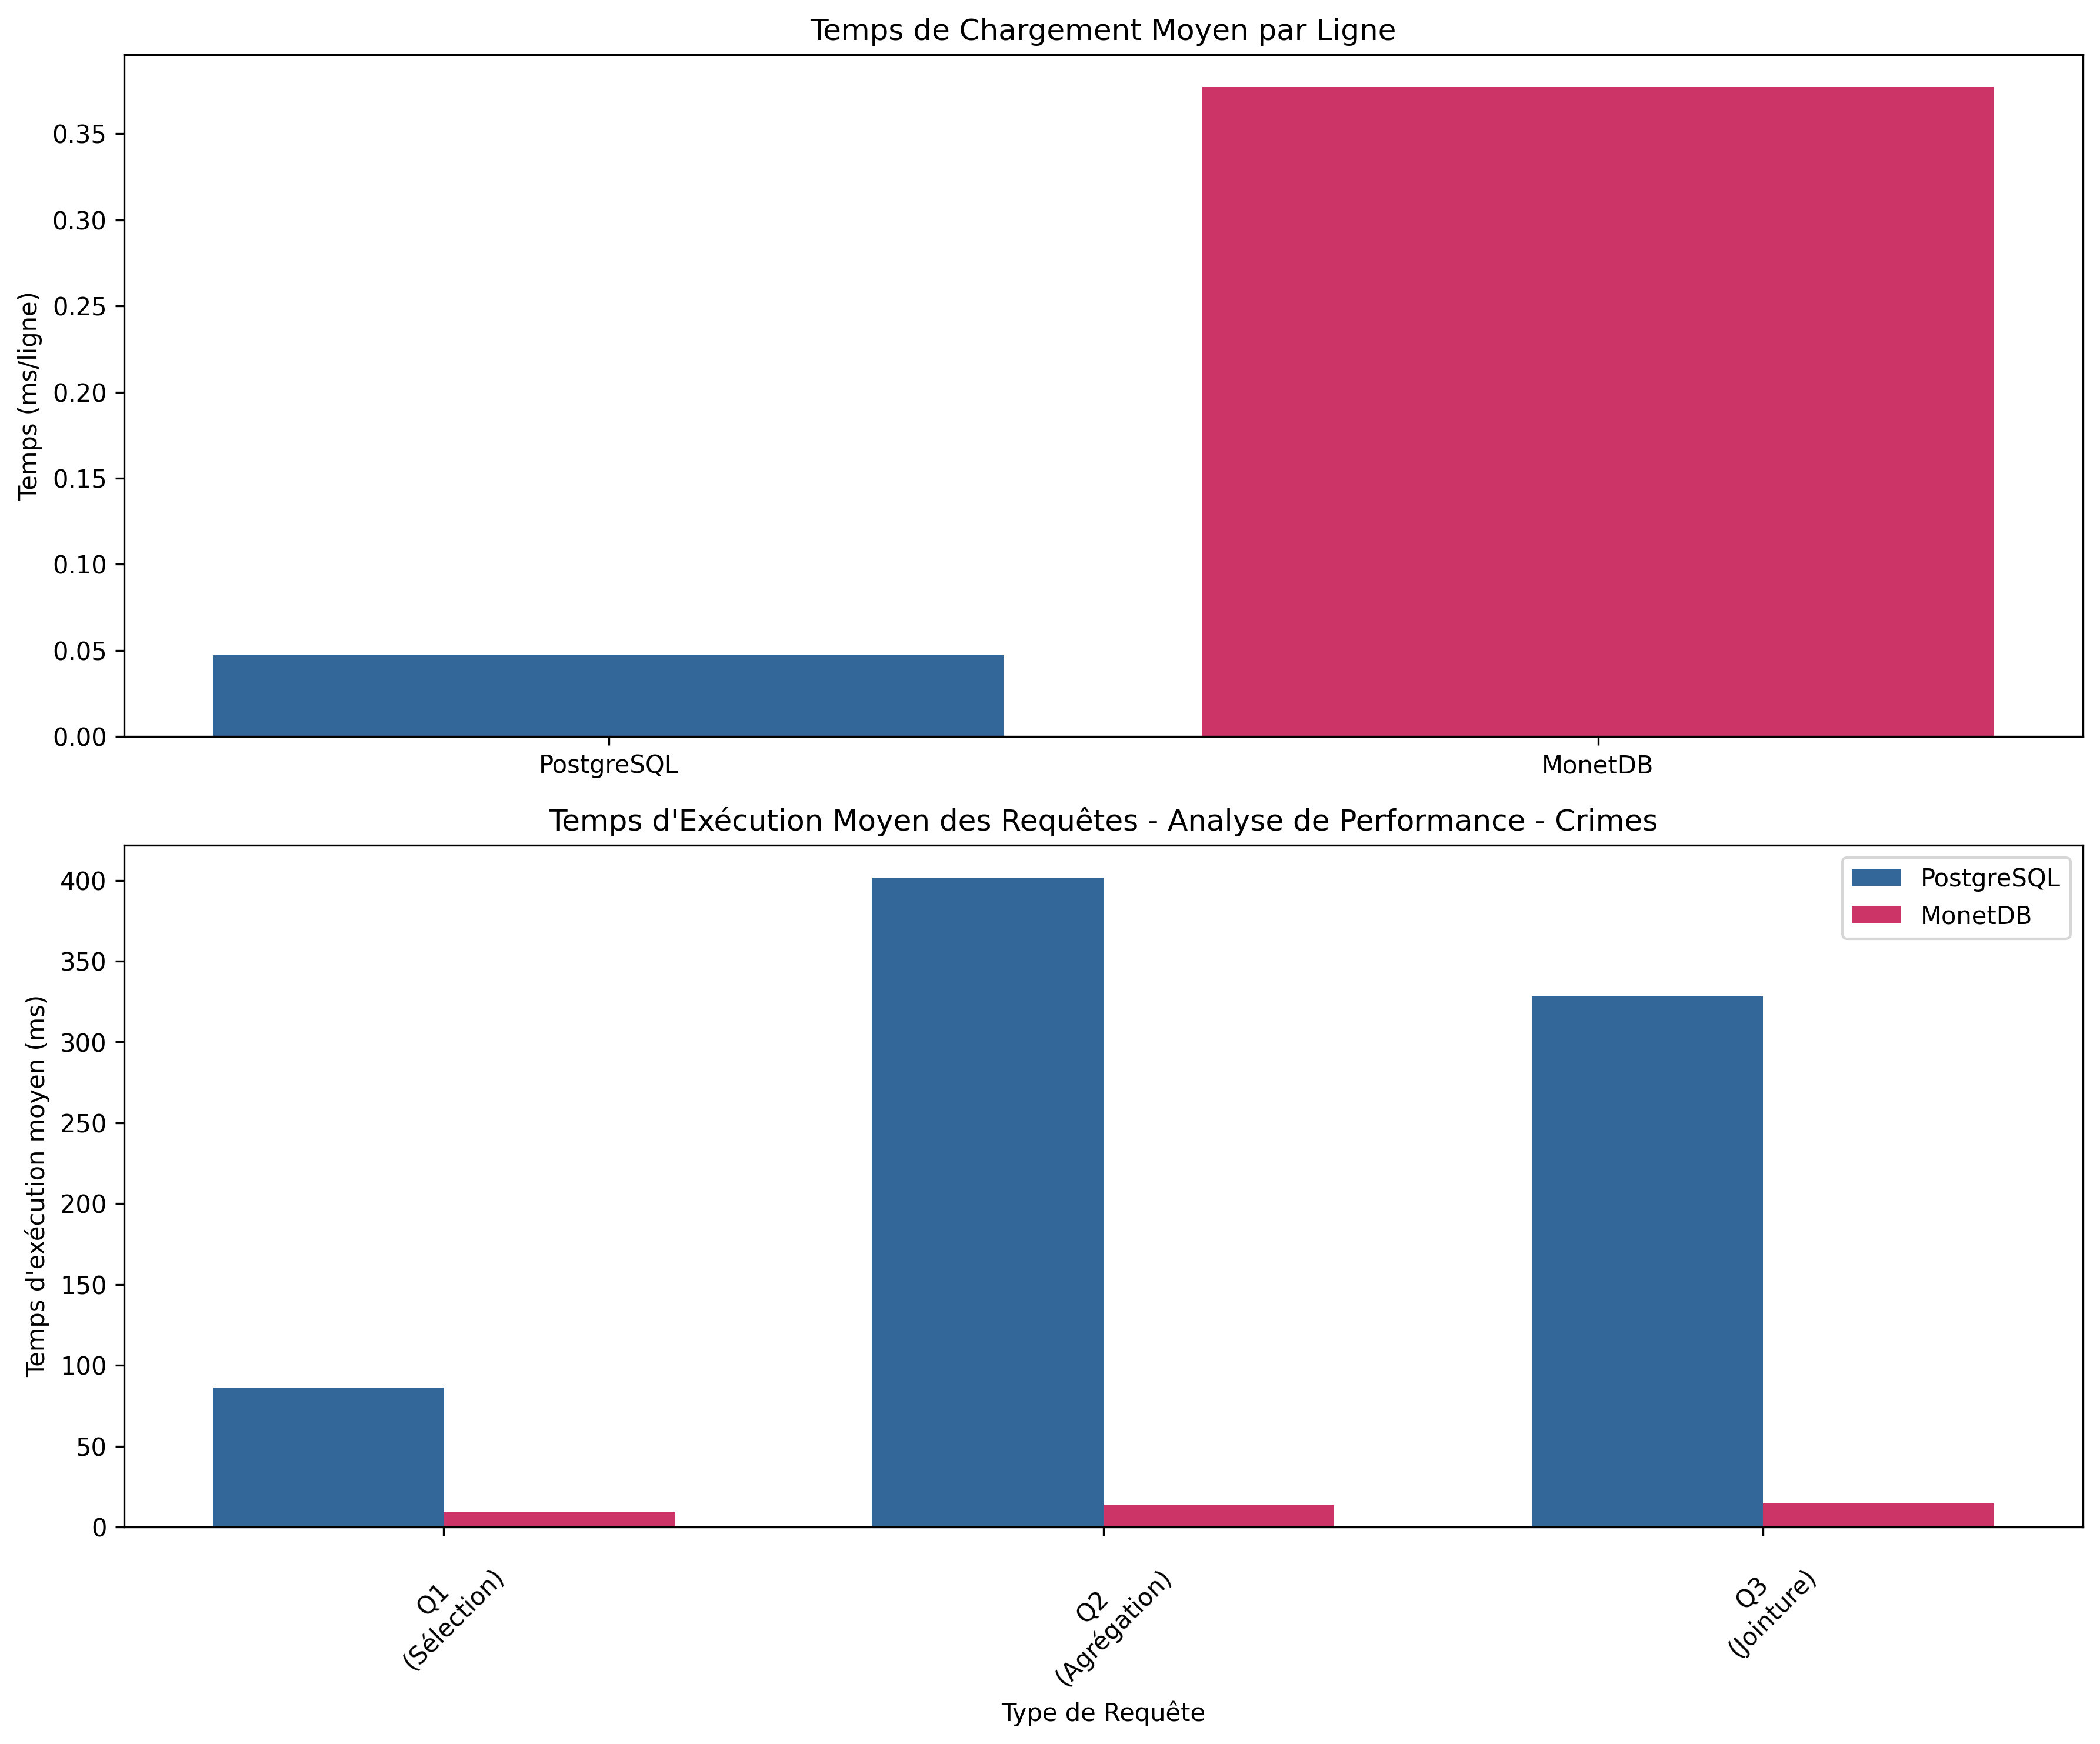
\includegraphics[width=0.8\textwidth]{images/crimes_performance.png}
      \caption{Analyse de Performance - Criminalité}
      \label{fig:performance_crimes}
  \end{figure}

\section{Conclusion}
\paragraph{}
Lors de la phase théorique, notre hypothèse était que MonetDB serait plus performant uniquement dans la grande base de données, et pour les requêtes de sélection, agrégation et jointures.
\paragraph{}
Comme on à pu le voir dans dans la partie expérimentale, ces résultats se sont, pour la plupart, confirmés. Néanmoins, pour le petit jeu de données, postgreSQL et MonetDB se valent en ce qui concerne les requêtes de sélections et d'agrégations. On peut alors se demander ce qui se passerait si la base de donnée que nous avions choisit était encore plus petite. Avec par exemple moins de 10 000 entrées. Peut-être que des différences plus marquantes auraient pu apparaître.
\paragraph{}
Enfin, on peut voir que les différences les plus significatives apparaissent en faveur de postgreSQL peu importe le nombre d'entrées en matière de chargement de données. Même chose pour MonetDB dans la grande base de données, pour les sélections, agrégations et jointures, les différences sont énormes.

\end{document}